\documentclass[vietnamese]{vlththesis}
\usepackage{tikz}
\usetikzlibrary{calc}
\newcommand{\comment}[1]{\ignorespaces}
\graphicspath{ {image/} }
%\addbibresource{bibbi.bib}
\makenoidxglossaries

\newacronym{lppl}{LPPL}{LaTeX Project Public License}
\newacronym{tex}{\TeX}{Tau Epsilon Chi}
\newacronym{wysiwyg}{WYSIWYG}{What you see is what you get}
\newacronym{ctan}{CTAN}{Comprehensive \TeX\ Archive Network}
\newacronym{ams}{AMS}{American Mathematical Society}
\newacronym{isbn}{ISBN}{International Standard Book Number}
\newacronym{lof}{LoF}{List of Figures}
\newacronym{lot}{LoT}{List of Tables}
\newacronym{toc}{ToC}{Table of Contents}
%opening
\title{Blockchain}
\author{Nguyễn Lễ}
\supervisorName{Nguyễn Anh Thư}

\makeatletter
\newcommand{\printtitlepage}{
	\thispagestyle{empty}
	\begin{center}
		{\bfseries\parskip=0pt
			
			\theGroup
			\vspace*{0.1cm}
			
			\theUniversity
			\vspace*{0.1cm}
			
			\theFaculty
			\vspace*{0.1cm}
			
			\theDepartment\\
			\vspace*{0.1cm}
			------------------oOo------------------
		}
		\vspace*{1cm}
		
		{\bfseries
			\large
			\theReport}
		
		\vspace*{2cm plus 1cm minus 0.5cm}
		
		\iftoggle{viet}
		{\begin{flushleft}
				\textsl{\Large\underline{Đề tài:}}
		\end{flushleft}}
		{~}
		{\huge\bfseries
			\textcolor{cstred}{\@title}\par	
		}
	\end{center}
	
	\vspace*{2cm plus 1 cm minus 0.5cm}
	
	\hfill
	{\bfseries\large
		\iftoggle{viet}{%
			\begin{tabular}{r l}
				\underline{SVTH}: & \@author\\
				\underline{CBHD}: & \thesupervisorName\\
			\end{tabular}%
		}{%
			\begin{tabular}{r l}
				\underline{Student}: & \@author\\
				\underline{Supervisor}: & \thesupervisorName\\
			\end{tabular}%
	}}
	
	\vfill
	\begin{center}
		-----------------------------------------\\
		\bfseries
		\thePlace\ - \theDate
	\end{center}
	\clearpage
	
	
}

\makeatother

\begin{document}

\begin{titlepage}
	
\begin{tikzpicture}[remember picture, overlay]
	\draw[line width = 2pt] ($(current page.north west) + (1.1in,-1.1in)$) rectangle ($(current page.south east) + (-0.5in,0.9in)$);
	\draw[line width = 2pt] ($(current page.north west) + (1.2in,-1.2in)$) rectangle ($(current page.south east) + (-0.6in,1in)$);
	\end{tikzpicture}
	\makeatletter
	\printtitlepage
	\makeatother
\end{titlepage}

\printcoverpage
\acknowledgements{Đầu tiên, con xin gửi lời biết ơn đến mẹ, người đã thay thế vai trò người cha đã mất, cáng đáng cả gia đình và nuôi
dưỡng con nên người, con cũng xin cảm ơn dì Chính, người mà còn vẫn luôn coi như người mẹ thứ hai, chăm sóc con từng
miếng ăn, giấc ngủ và luôn coi con như con ruột của mình, công ơn của hai mẹ dành cho con không từ ngữ nào mà diễn tả được.\par
Em xin cảm ơn các thầy cô khoa Vật Lý - Vật Lý Kĩ Thuật, đã tận tâm truyền đạt kiến thức cho em trong những năm đầu đại học.
Em xin chân thành cảm ơn thầy cô của Bộ môn Vật Lý Tin Học, đã xây dựng bộ môn với các trang thiết bị hiện đại và sự nhiệt
tình, thân thiện của các thầy cô, giúp em có thể thoái mái học tập, nghiên cứu mà không cảm thấy căng thẳng, áp lực. 
Những lời chỉ bảo của thầy cô đã cho em những kiến thức cần thiết và quý báu cho định hướng của mình.\par
Và em cũng xin gửi lời cảm ơn tới thầy TS. Nguyễn Chí Linh, đã giới thiệu và hướng em vào đề tài này khi em không xác định
được hướng đi cho mình, thầy cũng dành thời gian đọc, chỉnh sửa và góp ý cho bài báo cáo này được hoàn thiện hơn. Đồng thời
tôi cũng muốn cảm ơn những người bạn ở Vật Lý Lý Thuyết, đã dành thời gian với tôi trong những ngày mới bước vào chuyên ngành,
thông qua những buổi nói chuyện đó, tôi mới lần đầu biết đến nền tảng LaTeX.\par
Và cuối cùng, tôi xin cảm ơn những người bạn, những người đàn em đã cùng đồng hành với tôi trong suốt bốn năm trên giảng
đường Đại học, cảm ơn vì những khoảng khắc trò chuyện vui vẻ giúp giải toả áp lực đã trở thành một phần kỉ niệm của đời sinh viên.\par~\par
\hfill
\begin{minipage}[H]{0.5\textwidth}
 \centering
 \textsl{TP. Hồ Chí Minh, tháng 1 năm 2018.}\\
 \vspace{1cm}
 Trịnh Tích Thiện 
\end{minipage}
}
\printfrontmatter

\startintroduction
\fancyhead[L]{}
Ngày nay, ngoài các trình soạn thảo văn bản phổ biến, LaTeX cũng là một sự lựa chọn dành cho người soạn thảo được
tạo ra với triết lý hoàn toàn khác biệt so với các trình hiện hành. Nhận thấy hạn chế của chất lượng in ấn ở những
năm 1970, và việc người dùng tốn quá nhiều thời gian để định dạng thay vì tập trung soạn thảo, Donald E.Knuth đã phát
triển hệ thống TeX, và từ đó, Leslie Lamport xây dựng thành LaTeX, với mục đích giúp người dùng sử dụng câu
lệnh để việc thiết kế văn bản được thực hiện một cách tự động bởi hệ thống. \par 
Tuy xuất hiện đã lâu nhưng do không có tính trực quan vốn có của các trình soạn thảo văn bản thông thường cũng như đòi hỏi người sử dụng có khái niệm cơ bản, 
về ngôn ngữ đánh dấu (markup language), cộng thêm việc nền tảng này chỉ lưu hành trong giới học thuật, nên LaTeX vẫn
chưa thực sự phổ biến đến những người dùng phổ thông (mặc dù đối tượng sử dụng ngày càng đa dạng).\par
Nhận thấy LaTeX thích hợp để tạo các văn bản có quy chuẩn rõ ràng, đồng thời nền tảng cho phép người dùng thiết kế bố cục và kiểu văn bản
cho riêng mình, đề tài này đã ra đời nhằm mục đích thiết kế, xây dựng một mẫu báo cáo khoá luận chuẩn trên nền LaTeX, định nghĩa các câu lệnh
mới để hỗ trợ những người dùng sau này có thể dễ dàng định dạng các báo cáo khoá luận mà không tốn nhiều thời gian vào việc thiết kế, canh chỉnh, thay vào đó
tập trung hơn vào nội dung và thành phần văn bản của mình, kế thừa đúng với tinh thần của những người sáng tạo ra LaTeX.\par
Tài liệu về LaTeX tuy đa dạng, nhưng lại có tính chuyên môn, đòi hỏi thời gian tìm hiểu và tổng hợp những tài liệu thật sự cần thiết, nhưng cũng nhờ
đó, tôi đã có thêm kĩ năng đọc hiểu, tìm kiếm thông tin, đồng thời hiểu thêm được các khái niệm, thao tác lập trình với
macro, cũng như tiếp cận và biết thêm được nhiều thủ thuật soạn thảo, trình bày văn bản theo ý mình sử dụng LaTeX, và đó
là những lý do tôi chọn đề tài này. Thông qua đề tài, ngoài việc xây dựng thành công một mẫu khoá luận, tôi cũng
muốn phổ biến sự tiện lợi trong việc soạn thảo các văn bản khoa học của LaTeX đến nhiều người hơn bằng việc giới thiệu, đưa
ra những hướng dẫn cơ bản và tổng hợp những nguồn tham khảo tin cậy cho hệ thống LaTeX này.\par
Báo cáo đề tài gồm bốn chương chính như sau:\par
\clearpage 
\begin{itemize}
 \item \textbf{Chương \ref{ch:1}: Tổng quan về LaTeX.} Giới thiệu khái niệm của LaTeX và lịch sử hình thành của hệ thống, đồng thời giới
 thiệu sơ lược về trình soạn thảo hỗ trợ LaTeX.
 \item \textbf{Chương \ref{ch:2}: Soạn thảo văn bản trong LaTeX.} Hướng dẫn cách tải và cài đặt nền tảng LaTeX trên hai
 hệ điều hành Windows và Linux, đồng thời đưa ra những hướng dẫn cơ bản về cách soạn thảo văn bản bằng LaTeX, các khái niệm,
 thuật ngữ và câu lệnh cần nắm để dễ dàng hiểu được các tài liệu hướng dẫn LaTeX.
 \item \textbf{Chương \ref{ch:3}: Thiết kế định dạng văn bản riêng trong LaTeX.} Sẽ tập trung vào cách thức thiết kế các
 định dạng văn bản riêng trong LaTeX, từ đó tiến tới thiết kế bài báo cáo, luận văn, sau đó
 phân tích quy trình tạo và cấu trúc của tập tin (file) sản phẩm đề tài.
 \item \textbf{Chương \ref{ch:4}: Kết luận và hướng phát triển.} Đưa ra kết luận về kết quả thu được của đề tài này
 và đánh giá hướng phát triển của thành phẩm.
\end{itemize}

\fancyhead[L]{\slshape\nouppercase{\chaptertitlename\ \thechapter}}
\chapter{Khái quát về blockchain}\label{ch:1}
\section{Lịch sử}

Những ý tưởng đầu tiên về chuỗi các block bảo mật nhờ các phương pháp mã hóa được mô tả vào năm 1991 bởi hai nhà khoa học Stuart Haber và W. Scott Stornetta \cite{haber}. Vào năm 1992, Bayer, Haber và Stornetta tích hợp cây Merkle  vào thiết kế, giúp cải thiện tính hiệu quả bằng cách cho phép nhiều văn bản được gom chung vào một block \cite{cryptocurrencytech}.

Khái niệm về blockchain được trình bày lần đầu bởi một người (hoặc nhóm người) có bút danh Satoshi Nakamoto  vào năm 2008. Nó được hiện thực hóa vào năm tiếp theo bởi Nakamoto như một thành phần cốt lõi của đồng tiền ảo bitcoin, nơi blockchain hoạt động như một sổ ghi chép công cộng mọi giao dịch trên hệ thống mạng. Thông qua việc ứng dụng  blockchain, bitcoin trở thành đồng tiền ảo đầu tiên giải quyết được vấn đề trả-tiền-hai-lần mà không cần đến một một bên được ủy quyền
và là nguồn cảm hứng cho  nhiều ứng dụng khác.

Tháng Tám năm 2014, kích thước file của blockchain bitcoin, chứa ghi chép của tất cả giao dịch diễn ra trên hệ thống mạng, đạt 20 GB. Vào tháng Một năm 2015, kích thước file đã tăng lên đến gần 30 GB, và từ tháng Một 2016 đến tháng 2017, blockchian bitcoin đã tăng từ 50 GB lên 100 GB về kích thước.

Từ \textit{block} và \textit{chain} được sử dụng một cách riêng rẻ trong tài liệu gốc của Satoshi Nakamoto, nhưng dần dần trở nên phổ biến như một từ đơn, \textit{blockchan}, vào năm 2016. Thuật ngữ blockchain 2.0 chỉ những ứng dụng mới của cơ sở dữ liệu blockchain phân tán, nổi lên lần đầu vào năm 2014. Tạp chí \textit{The Economist} mô tả \textit{Ethereum}, một ứng dụng của blockchain có khả năng lập trình thế hệ thứ hai này như sau: "một ngôn ngữ lập trình cho phép người dùng viết ra những hợp đồng thông minh phức tạp hơn, nhờ đó tạo ra những hóa đơn tự trả khi một đơn hàng tới hay tự động chia cổ tức cho cổ đông khi lợi nhuận đạt tới một mức nhất định". Công nghệ Blockchain 2.0 đã vượt ra khỏi khuôn khổ giao dịch và cho phép  "trao đổi giá trị mà không cần tới những bên trung tâm đầy quyền lực hoạt động như những kẻ kiểm soát tiền và thông tin". Chúng được mong đợi sẽ cho phép mọi người tham gia vào nền kinh tế toàn cầu, bảo vệ qyền riêng tư của những người tham gia, cho phép mọi người "kiếm tiền từ thông tin của chính họ" và cung cấp khả năng đảm bảo những người tạo ra nội dung được trả thưởng  cho tài sản trí tuệ họ làm ra. Công nghệ blockchan thế hệ thứ hai cho phép lưu trữ "ID số và diện mạo thay đổi liên tục" của từng cá nhân và cung cấp giải pháp giải quyết vấn đề bất bình đẳng xã hội bằng cách "thay đổi cách thức của cải được phân phối". 

Vào năm 2016, Kho lưu ký chứng khoán trung tâm của Liên bang Nga (NSD) đã công bố một dự án thí điểm, dựa trên nền tảng blockchian 2.0 Nxt nhằm khai thác và đưa vào sử dụng hệ thống bầu cử tự động dựa trên nàng blockchain. IBM đã mở môt trung tâm nghiên cứu đổi mới blockchain tại Singapore vào tháng Bảy năm 2016. Một nhóm làm việc cho Diễn đàn Kinh tế Thế giiới đã gặp nhau vào tháng 11 năm 2016 để thảo luận sự phát triển các mô hình quản trị liên quan đến blockcchain. Theo Accenture, một ứng dụng của lý thuyết khuyến đại cải tiến (Diffusion of innovations), cho rằng blockchain đạt tỉ lệ 13,5\% ứng dụng trong các dịch vụ tài chính năm 2016,. Các nhóm thương mại công nghiệp đã tham gia tạo ra Diễn đàn Blockchain thế giới, một sáng kiến của Phòng Thương mại Số Hoa Kỳ. 

\section{Double Spending: Vấn đề mà blockchain giải quyết}
Trong suốt chiều dài lịch sử, các loại tiền tệ bằng kim loại hoặc giấy được sử dụng bởi nhiều nền văn minh trên khắp thế giới. Trong các giao dịch được thực hiện với các loại tiền ấy, một bên phải trả một lượng tiền cho bên thứ hai để nhận một lượng hàng hóa hoặc dịch vụ. Khi tiền thực được trao đổi, không có khả năng cùng một món tiền lại được trả bởi cùng một bên hai lần.

Ví dụ, với các loại tiền giấy hoặc kim loại, một người không thể trả một đô la cho một quả táo, và sau đó sử dụng  đúng đồng đô la đó để mua quả cam. Đó là vì  đồng đô la đã được chuyển cho người bán trong quá trình mua bán quả táo. Tuy nhiên, với tiền ảo, không có quá trình chuyển vật lý của tiền, tạo nên cái được goi là vấn đề vấn đề trả tiền hai lần.

vấn đề trả tiền hai lần là khi một người dùng cùng một món tiền cho hai giao dịch hoặc nhiều hơn. Trước khi có Bitcoin, đây là một vấn đề lớn vì nó xóa bỏ đặc trưng giới hạn về số lượng của các loại tiền ảo, vốn là đặc trưng cơ sở để một loại tiền để có thể tồn tại. Nếu mỗi đơn vị tiền có thể được dùng một lượng vô hạn số lần, thì nó sẽ không có giá trị thực nào.

\section{Theo bước Satoshi Nakamoto}

Sau cuộc khủng hoảng tài chính 2008, một nhà tiên phong tên Satoshi Nakamoto đã tìm ra cách giải quyết cho  vấn đề vấn đề trả tiền hai lần và tạo ra một loại tiền ảo không bị vấn đề trả tiền hai lần ảnh hưởng. Cho đến nay, không ai biết được danh tính thật sự của Satoshi. Satoshi Nakamoto chỉ là một bút danh.

Satoshi Nakamoto đã tạo ra một giải pháp độc nhất để ngăn chặn double sending. Giải quyết đó được goi là công nghệ blockchain. Chi tiết của cả Bitcoin và công nghệ blockchain được trình bày trong một sách trắng được phát hành bởi Satoshi Nakamoto vào tháng 11 năm 2008 tên là "Bitcoin: A Peer-to-Peer Electronic Cash System". 

Trong sách trắng này, Nakamoto giải thích tại sao các giao dịch tài chính điện tử lúc đó vẫn phải phụ thuộc vào bên thứ ba được tin cậy (ví dụ như ngân hàng) để giải quyết vấn đề vấn đề trả tiền hai lần, và việc đó có thể được thay đổi với công nghệ blockchain ra sao.

\section{Công nghệ blockchain}

Công nghệ blockchain về cơ bản là một sổ cái công cộng ghi chép mọi giao dịch trên một bản ghi có thể mở rộng. Các giao dịch phải được chứng thực bởi các "thợ đào" để chúng được coi là hợp lệ và được thêm vào blockchain. Các thợ đào nhận được những khuyến khích để thực hiện việc chứng thực - một lượng Bitcoin nhất định cho một lần chứng thực giao dịch thành công.

Với phương thức này, ta không cần tới ngân hàng để ngăn chặn vấn đề trả tiền hai lần và mỗi giao dịch đều được xác minh để đảm bảo rằng không ai xài cùng một lượng Bitcoin quá một lần. Nếu có ai đó tìm cách xài cùng một lượng Bitcoin hai lần bằng cách thực hiện hai giao dịch khác nhau với cùng một đầu vào Bitcoin trên cùng một block, thì hai giao dịch sẽ không bao giờ được xác nhận trên hệ thống mạng. Nhờ đó mà cơ bản biến chúng thành các giao dịch không hợp lệ và chúng sẽ bị "hủy", qua đó ngăn chặn vấn đề trả tiền hai lần.

Các chi tiết về việc làm thế nào mà blockchain có thể ngăn chặn được vấn đề trả tiền hai lần sẽ được trình bày ở các chương sau, liên quan đến cấu trúc dữ liệu của nó và các phương pháp mã hóa được ứng dụng trong công nghệ blockchain.

\section{Các loại blockchain}
Một blockchain có thể thuộc loai không cần cho phép (permissionless) ,như Bitcoin hoặc Ethereum; hoặc cần cho phép (permissioned). Một blockchain không cần cho phép, còn được gọi là một blockchain công cộng bởi vì bất kỳ ai đều có thể tham gia vào mạng. Một blockchain cần cho phép, hay blockchain riêng tư, yêu cầu có sự xác minh trước của các bên tham gia trong mạng, và các bên này thường đã biết nhau.

Sự lựa chọn giữa blockchain công cộng và riêng tư thường được quyết định bởi các ứng dụng cụ thể cần giải quyết. Một ví dụ mà các doanh nghiệp trao đổi thông tin với nhau là trong quản lý chuỗi cung ứng. Quản lý chuỗi cung ứng là một trường hợp lý tưởng để sử dụng blockchain riêng tư. Ta không muốn các công ty không mời tham gia vào mạng. Mỗi bên tham gia chuỗi cung ứng sẽ được yêu cầu quyền (permission) để thực hiện các giao dịch trong blockchain. Các giao dịch này sẽ cho phép các công ty khác biết một sản phẩm cụ thể đang nằm ở đâu.

Ngược lại, khi một mạng có thể tạo thuận lợi cho các bên giao dịch mà không nhất thiết phải xác minh danh tính của nhau, như blockchain Bitcoin, một blockchain công cộng phù hợp hơn. Một số ví dụ như bán hoặc phân phối sản phẩm trong một cộng đồng. Các loại tiền mã hóa (vốn không được các chính phủ ủng hộ) thường sử dụng blockchain công cộng.

\section{Sự cần thiết của blockchain}

\chapter{Cách thức hoạt động của blockchain}
\comment{
\section{Mật mã Chìa Khóa Bất đối xứng}

Mật mã bất đối xứng (Asymmetric cryptography), hay còn gọi là mật mã công cộng (public cryptography) là một thành phàn nền tàng của blockchain và các loại tiền ảo như Bitcoin và Ethereum. Những kỹ thuật mật mã nâng cao này đảm bảo rằng nguồn gốc của giao dịch là hợp lệ và các tin tặc không thể đánh cắp tiền của người dùng.

\subsection{Khái niệm}
Mật mã bất đối xứng luôn sử dụng hai chìa khóa: văn bản được mã hóa bằng một trong hai chìa khóa chỉ có thể được giải mã với chìa khóa kia, và ngược lại. Khi sử dụng mật mã bất đối xứng trong thực tế, các chìa khóa này được gọi là chìa khóa công cộng và chìa khóa riêng tư để làm nổi bật vai trò của chúng. Chìa khóa công cộng đựoc chia sẽ cho mọi người, trong khi chìa khóa riêng tư được giữ bí mật.  Vì lí do này, mật mã bất đối xứng còn được gọi là mật mã chìa khóa công cộng - riêng tư.

Hai trường hợp sử dụng cơ bản của chìa khóa công cộng và cổ điển là:

\begin{itemize}
	\item Mọi người đều có thể sử dụng chìa khóa công cộng để mã hóa dữ liệu mà say đó chỉ có thể được giải mã bởi người nám giữ chìa khóa riêng tư tương ứng. Điều này tương đồng với một hộp thư công cộng nơi mọi người có thể cho thư vào nhưng chỉ có chủ sở hữu có thể mở nó.
	\item Người nắm giữ chìa khóa riêng tư có thể sử dụng nó để mã hóa sử dụng dữ liệu mà sau đó chỉ có thể được giải mã bởi những người sở hữu chìa khóa công cộng tương ứng, Điều này tương đồng với một bảng thông báo công cộng nơi những ai có bản sao chép của chìa khóa công cộng có thể đọc tin nhắn nhưng chỉ người nắm giữ chìa khóa riêng tư có thể tạo ra tin nhắn
\end{itemize}

Blockchain sử dụng mật mã bất đối xứng nhằm đạt được hai mục địch:
\begin{itemize}
	\item Xác định tài khoản: Tài khoản người sư dụng là chìa khóa mật mã công cộng.
	\item Xác thực giao dịch: Chủ sở hữu của tài khoản, người nằm giữ quyền sở hữu tài sản, tạo ra một văn bản được mã hóa với chìa khóa riêng tư tương ứng. Văn bản được mã hóa này có thể được chứng thực bằng cách sử dụng chìa khóa công cộng tương ứng, chính là số tài khoản chủ sở hữu.
\end{itemize}

\section{Chữ ký điện tử}

Trong thế giới thực, chữ ký viết tay trên văn bản tuyên bố sự đồng thuận của tác giả với nội dung của văn bản đã ký. Khả năng chứng minh của chữ ký bằng nay dựa trên sự độc nhất của chữ  viết tay của mỗi người.

Chữ ký điện tử là phiên bản điện tử tương đờng của chữ ký viết tay, Nó phục vụ hai mục đích:
\begin{itemize}
	\item Xác thực tác giả duy nhất
	\item Tuyên bố sự đồng thuận của tác giả với nội dung văn bản và xác thực những điều được thực thi trong đó.
\end{itemize}

Trong blockchain, chữ ký điện tử của các giao dịch chính là mã băm mật mã của dữ liệu giao dịch được mã hóa bằng chìa khóa riêng tư tương ứng với tài khoản người nắm quyền sở hữu. 


\subsection{Khái niệm mã băm}
Nói một cách đơn giản, băm nghĩa là lấy một chuỗi đầu vào với độ dài bất kỳ và cho đầu ra là một chuỗi với độ dài cố định. Trong phạm vi tiền ảo như Bitcoin, các giao dịch được lấy làm đầu vào và chạy qua một thuật toán băm (Bitcoin sử dụng SHA-256) cho một đầu ra là chuỗi có độ dài cố định.
Ta có ví dụ như bảng 3.1. 

Trong trường hợp của SHA-256, bất kể đầu vào có lớn hay nhỏ đến đâu, đầu ra sẽ luôn có độ dài cố định 245-bit. Điều này trở nên quan trọng khi ngày nay, khối lượng dữ liệu và giao dịch cần xử lý ngày một lớn dần. Do đó, thay vì phải nhớ dữ liệu đầu vào, ta chỉ cần nhớ mã hash của nó để tiện theo dõi.

\subsection{Hàm băm mật mã học}
Hàm băm mật mã học (cryptographic hash function) là một lớp đặc biệt của hàm băm. Nó csubó những tính chất khác nhau khiến nó trở nên lý tướng để áp dụng trong lĩnh vực mã hóa.  

Một hàm băm mật mã học lý tưởng có những tính chất chính sau:
%Tất định: các tin nhắn giống nhau luôn có cùng mã băm.
%Nhanh chóng tính ra mã băm với mọi tin nhắn được cung cấp.
%Không thể tạo lại tin nhắn từ mã băm của nó, ngoại trừ bằng cách thử mọi tin nhắn khả dĩ
%Một thay đổi nhỏ trong tin nhắn cũng dẫn đến thay đổi mã băm của nó một cách sâu rộng, dẫn đến mã băm mới không có tương quan gì sao với mã băm cũ.
% Không thể tìm được hai tin nhắn khác nhau có cùng mã băm.


\textbf{Tính chất 1: Tất định}

Các tin nhắn giống nhau luôn có cùng mã băm.

\textbf{Tính chất 2: Tính nhanh}

Hàm băm phải có khả năng đưa ra mã hash của đầu vào một cách nhanh chóng. Nếu tiến trình không đủ nhanh thì hệ thống sẽ không hiệu quả

\textbf{Tính chất 3: Pre-Image Resistance}

Tính chất này nói rằng nếu được cho trước mã hash h, sẽ rất khó khăn để tìm được tin nhắn m thỏa h = hash(m). Khái niệm này liên quan đến tính chất của hàm một chiều.

\textbf{Tính chất 4: Thay Đổi Nhỏ ở Đầu Vào Dẫn Đến Thay Đổi Toàn Bộ Mã Hash}

Kể cả nếu ta chỉ gây một thay đổi nhỏ ở đầu vào, thay đổi được phản ánh ở mã hash mới sẽ rất lớn. Ví dụ sử dụng SHA-256:

%\begin{table}[h!]
%	\begin{tabu} to\linewidth{ |X[2] | X[8] | }
%		\hline
%		Input & Hash \\
%		\hline
%		This is a test & \seqsplit{C7BE1ED902FB8DD4D48997C6452F5D7E509FBCDBE2808B16BCF4EDCE4C07D14E} \\ \hline
%		this is a test & \seqsplit{2E99758548972A8E8822AD47FA1017FF72F06F3FF6A016851F45C398732BC50C} \\ \hline
%		
%	\end{tabu}
%	\centering
%	
%	\caption[Table caption text]{Ví dụ tác động của thay đổi đầu vào}
%\end{table}

Đây là một tính chất quan trọng vì nó sẽ dẫn đến một trong những đặc tính quan trọng nhất của blockchain, tính không thể thay đổi.

\textbf{Tính chất 5: Collision Resistant}

Một xung đột xảy ra khi hai đầu vào khác nhau tạo ra cùng một đầu ra. Một hàm băm H có tính khá xung đột nếu không ai có thể tìm được một xung. Biểu đạt một cách hình thức thì:

Một hàm băm H được cho là kháng xung đột nếu như khó khả thi để tìm hai giá trị, x và y,  với x $\neq$ y sao cho H(x) = H(y)

%Ta nói rằng "không ai có thể tìm được" một xung đột, nhưng ta không nói rằng không có xung đột nào tồn tại. Thực tế, xung đột tồn tại trong bất cứ hàm băm nào, 

 \begin{figure}[h]
	\centering	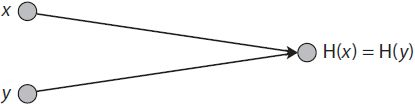
\includegraphics[width=0.9\textwidth]{collision}
	\caption{Một xung đột hàm băm, x và y là hai giá trị khác biệt, nhưng khi truyền vào hàm băm H, chúng tạo ra cùng đầu ra}
\end{figure}

\textbf{Tính chất 6: Puzzle friendliness}

Một hàm băm H được cho là puzzle friendly nếu với mọi giá trị đầu ra y, nếu k được chọn là một phân phối với  high min-entropy, khó khả thi để tìm được một đầu ra x thỏa H(k|x) = y.


% \section{Mã hóa}
% \subsection{Mật mã đối xứng}
% Với mật mã đối xứng (hoặc mã hóa chìa khóa-đồng bộ), cùng một chìa khóa được sử dụng cho cả quá trình mã hóa và giải như được thể hiện trong hình 
%
% Mật mã đối xứng có hai loại
% Stream Ciphers.
% Block Ciphers.
%
% Stream Ciphers
% Stream Ciphers nghĩa là sử dụng một chìa khóa có độ dài cố định nhằm thay thế tin nhắn với một chuỗi kí tự giả ngẫu nhiên (pseudorandom). Về cơ bản, nó mã hóa từng chữ cái của tin nhắn .
%
% 3 dạng của stream ciphers:
%
% One-time pad với bảng chữ cái
% Để thực hiện dạng mã hóa này cần có một chìa khóa có cùng số kí tự với tin nhắn và nó chỉ có thể được sử dụng một lần duy nhất.
%
% GIả sử A  gửi tin nhắn “MEET ME OUTSIDE” đến Bob. Nhưng A không muốn ai chặn tin nhắn của họ. Vì vậy, A và Bob quyết định sử dụng một one-time pad 
%
%
% Quá trình mã hóa

\subsection{Mật mã bất đối xứng}

mã hóa bất đối xứng, sử dụng một cặp chìa khóa có liên quan với nhau về mặt toán học, một chìa công khai dùng để mã hoá (public key) và một chìa bí mật dùng để giải mã (private key) như hình \ref{fig:asymmetric}. Một thông điệp sau khi được mã hóa bởi chìa công khai sẽ chỉ có thể được giải mã với chìa bí mật tương ứng. Do các thuật toán loại này sử dụng một chìa khóa công khai (không bí mật) nên còn có tên gọi khác là public-key cryptography (thuật toán mã hóa dùng chìa khóa công khai).
 \begin{figure}[ht]
	\centering
	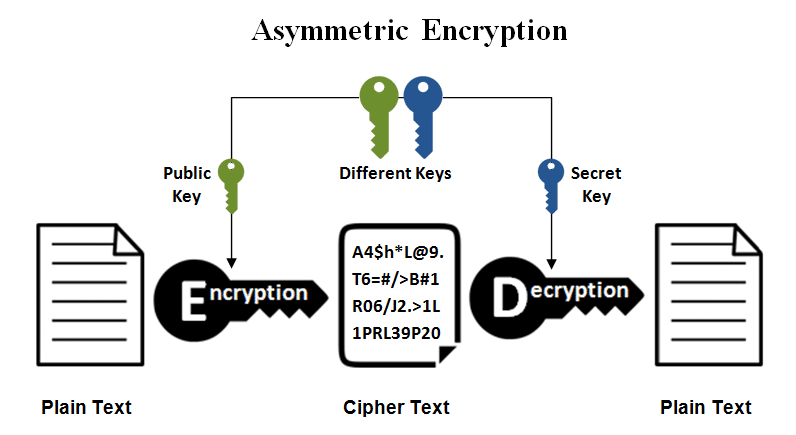
\includegraphics[width=0.9\linewidth]{image/asymmetric_cryptography}\label{fig:asymmetric}
	\caption{Minh họa mật mã bất đối xứng}
\end{figure}


Mật mã bất đối xứng có hai ứng dụng thực tế là:
Thuật toán Rivest-Shamir-Adleman (RSA).
Elliptical Curve Cryptography.}

\section{Mật mã trong blockchain}
Mật mã học là những phương pháp giúp che giấu và lộ diện, hay còn gọi là mã hóa và giải mã, thông tin thông qua các phương pháp toán học phức tạp. Điều này có nghĩa là thông tin không thể được xem bởi bất kỳ ai ngoại trừ  những người nhận được định trước. Các phương pháp bao gồm lấy các thông tin chưa được mã hóa như một đoạn văn bản, và mã hóa nó bằng cách sử dụng một thuật toán (tiếng Anh gọi là cypher).
Nó tạo nên một văn bản đã mã hóa (ciphetext), một mẩu thông tin hoàn toàn vô dụng và vô nghĩa chi đến khi được giải mã. Phương pháp mã hóa này được gọi là mã hóa chìa khóa đối xứng (symmetric-key cryptography).

Một ví dụ về mật mã xuất hiện sớm trên thế giới là mật mã Caesar (Caesar cipher), được sử dụng bởi Julius Caesar để bảo vệ các bí mật quan sự  của Roman. Mỗi chữ  cái trong một tin nhắn được thay thế với chữ cái đứng trước nó 3 chữ cái về phía bên trái trong bảng chữ cái, thông tin này về cơ bản chính là chìa khóa để giải mã tin nhắn. Các tướng của Caesar biết rằng để giải (decode) các chữ cái họ chỉ phải dịch mỗi chữ về phía phải (bảng chữ cái) ba lần, trong khi thông tin sẽ được giữ an toàn nếu bị chặn bởi kẻ thù của Caesar. Mật mã học hiện đại hoạt động tương tự, nhưng với độ phức tạp cao hơn rất nhiều.

 \begin{figure}[ht]
	\centering
	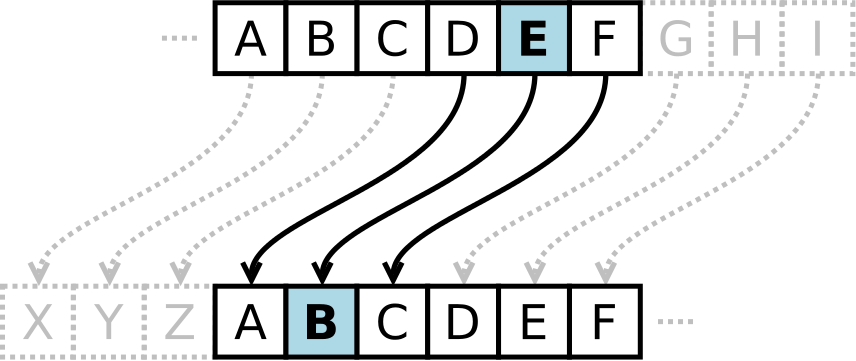
\includegraphics[width=0.9\linewidth]{image/Caesar_cipher_left_shift_of_3}\label{fig:Caesar}
	\caption{Cách thức hoạt động của một mật mã Caesar là thay thế mỗi chữ cái với một chữ khác cách một khoảng cố định trên bảng chữ cái}
\end{figure}

 \begin{figure}[ht]
	\centering
	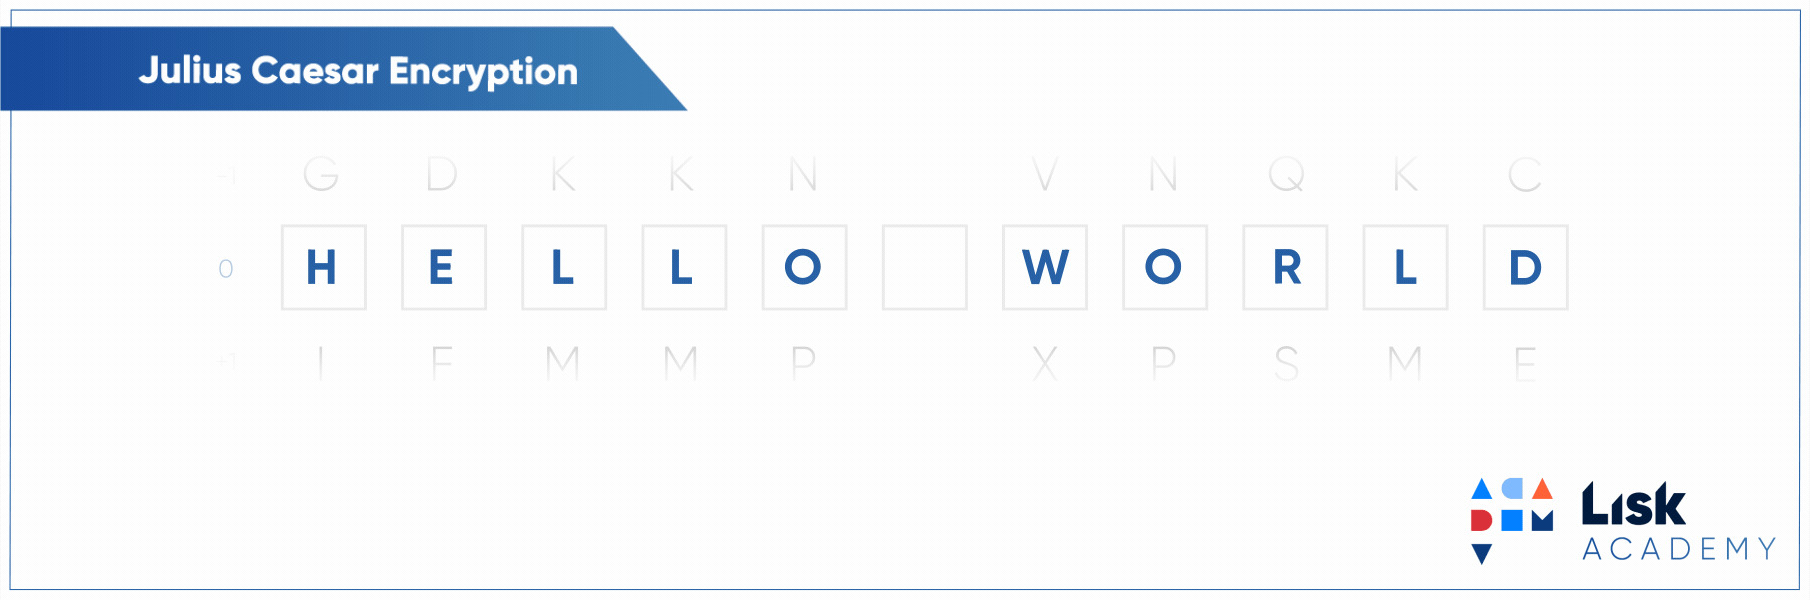
\includegraphics[width=0.9\linewidth]{image/caesarBefore}\label{fig:CaesarBefore}
	\caption{Câu "Hello World" trước khi mã hóa}
\end{figure}

\begin{figure}[ht]
	\centering
	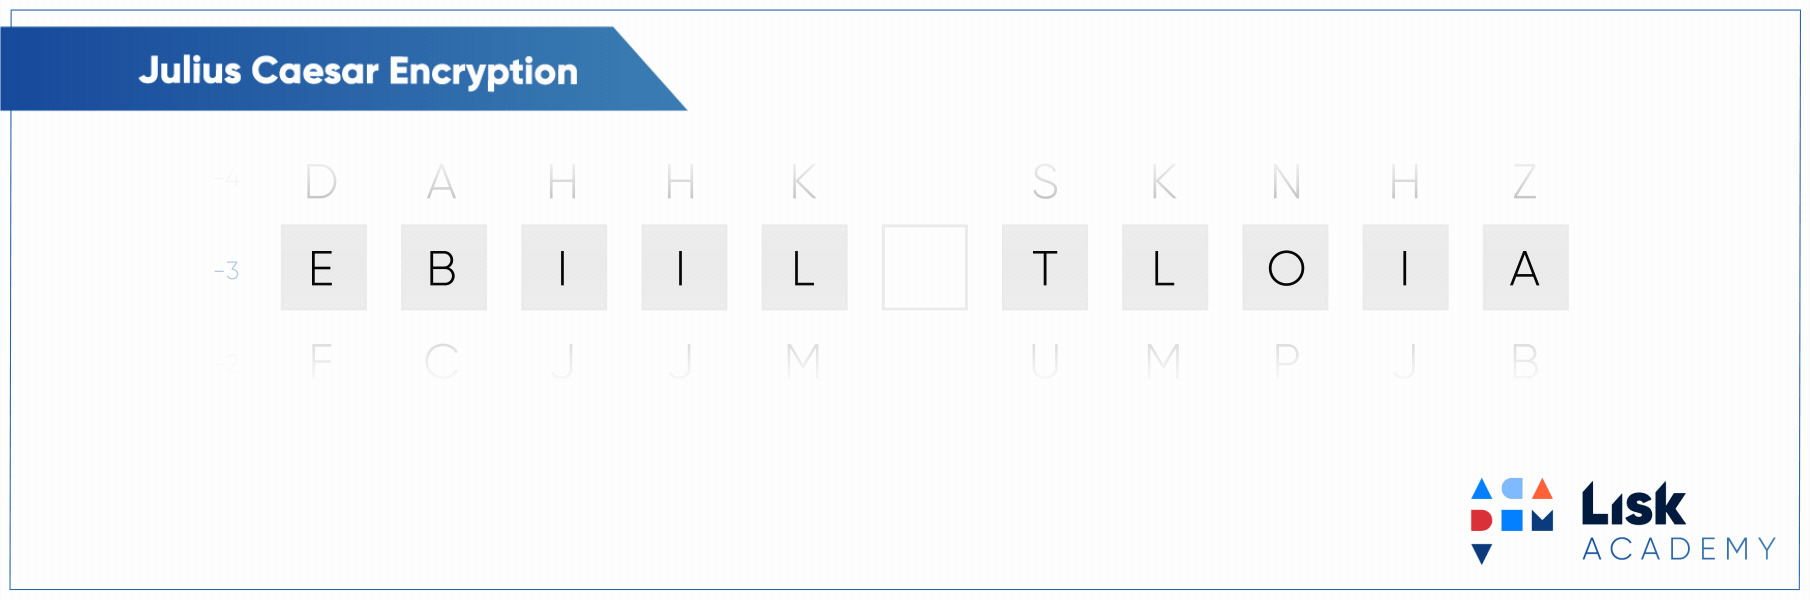
\includegraphics[width=0.9\linewidth]{image/caesarAfter}\label{fig:CaesarAfter}
	\caption{Câu "Hello World" sau khi mã hóa bằng mật mã Caesar}
\end{figure}


Mã nền (codebase) của phần lớn các thuật toán dùng trong mật mã là các dự án mã nguồn mở, nghĩa là code của chúng có thể được xem xét bởi bất kì ai. Thuật toán (cipher) được sử dụng rộng rãi nhất trên thế giới là AES, cho phép bất kì ai đều có thể sử dụng và code của nó được mở để cộng đồng có thể xem. Kết quả là nó đã được nghiên cứu chi tiết và cho đến nay chưa có lỗ hỗng nào được phát hiện.  Thuật toán này cũng được sử dụng bởi NSA, cơ quan tình báo Hoa Kỳ, như một công cụ được chọn để mã hóa thông tin. Vì vậy, có thể nói thông tin được ghi lại trên blockchain được bảo mật với cùng mức độ như bảo mật những bí mật nhạy cảm nhất thế giới. 

Trong blockchain, mật mã được sử dụng chủ yếu cho hai mục đích:
Bảo vệ nhận dạng (identities) của người gửi giao dịch
Đảm bảo các ghi chép trong quá khứ không thể bị giả mạo

Công nghệ blockchain sử dụng mật mã như một phương tiện để bảo vệ nhận dạng của người dùng, đảm bảo giao dịch được thực hiện một cách an toàn và bảo mật mọi thông tin và giá trị lưu trữ. Vì vậy, bất kì ai sử dụng blockchain đều có thể hoàn toàn tự tin rằng thông tin khi đã được ghi trên blockchain thì hoàn toàn hợp lệ và bảo mật.

Mặc dù được xây dựng trên một khuôn khổ tương tự, nhưng mật mã khóa công khai (public-key cryptography), loại mật mã được dùng trong blockchain, phù hợp với các chức năng liên quan đến blockchain hơn so với mật mã khóa đối xứng.

 Public-Key Cryptography, còn được gọi là asymmetric cryptography là một cải tiến trên nền tảng mật mã khóa đối xứng chuẩn: nó cho phép thông tin được truyền nhờ vào một khóa công khai có thể được chia sẽ với bất kỳ ai
 
 Thay vì sử dụng một chìa khóa duy nhất cho cả việc mã hóa và giảm mã, như với trường hợp của mật mã khóa đối xứng, trong mật mã khóa công khai, các chìa khóa riêng rẽ (một khóa công khai và một khóa riêng tư) được sử dụng.
 
 Sự kết hợp giữa khóa công khai và riêng tư của người dùng giúp mã hóa thông tin, còn khóa riêng tư của người nhận và khóa công khai của người gửi giúp giải mã nó. Không thể tìm ra khóa riêng tư dựa trên khóa công khai. Vì vậy, một người dùng có thể gửi khóa công khai của họ đến bất kỳ ai mà không sợ rằng ai đó sẽ có quyền truy cập vào khóa riêng tư của họ. Người gửi có thể mã hóa tập tin và chắc chắn rằng những tập tin đó sẽ chỉ có thể bị giải mã bởi bên được định trước.
 
 Thêm vào đó, thông qua mật mã khóa công khai, một chữ ký điện tử được tạo ra, bảo vệ sự toàn vẹn của dữ liệu. Điều này được thực hiện bằng cách kết hợp chìa khóa riêng tư của người dùng với dữ liệu mà họ muốn kí, thông qua thuật toán nhất định.
 
 Do bản thân dữ liệu là một phần của chữ kí số, hệ thống mạng sẽ không ghi nhận nó là hợp lệ nếu bất kì phần nào của nó bị giả mạo.  Việc chỉnh sửa kể cả nhỏ nhất cũng sẽ làm thay đổi toàn bộ chữ kí, làm cho nó sai khác đi và không dùng được nữa. Thông qua đó, công nghệ blockchain có khả năng đảm bảo rằng bất kì dữ liệu nào đã được ghi vào là đúng, chính xác và không bị giảm mạo. Chữ kí số tạo nên tính bất khả đổi của dữ liệu được khi trong một blockchain.
 
 \section{Chữ kí số}
 
Chữ kí số đúng như tên gọi của nó: nó cung cấp sự xác nhận và chứng thực tương tự như chữ kí bình thường, ở dạng số hóa. Phân đoạn này sẽ thảo luận cách chúng hoạt động cũng như cách đa chữ kí (multisignatures) được sử dụng để tăng thêm một lớp bảo mật.
 
Chữ kí số là một trong những phương tiện chính để đảm bảo tính an toàn và toàn vẹn của dữ liệu được ghi trên một blockchain. Chúng là một bộ phận tiêu chuẩn trong giao thức blockchain, được dùng chủ yếu để bảo vệ giao dịch và khối giao dịch, sự chuyển các thông tin nhạy cảm, phân phối phần mềm, quản lý hợp đồng và các trường hợp khác khi việc phát hiện và ngăn chặn các  hành động làm giả mạo từ bên ngoài. Chữ ký số sử dụng mật mã bất đồng bộ, nghĩa là thông tin có thể được chia sẽ với bất kỳ ai bằng cách sử dụng chìa khóa công khai.
 
 Ở nhiều nơi trên thế giới, chữ ký điện tử có cùng ràng buộc pháp lý như chữ kí thường. Ví dụ về các quốc gia và thực thể  công nhận chúng bao gồm: Liên Minh Châu Âu, Liên Hợp Quốc, Liên Hợp Quốc, Hoa Kỳ, Brazil, Mexico, India, Indonesia, Turkey và Saudi Arabia.
 
 Chữ kí số cung cấp ba lợi thế cho việc lưu trữ và truyền thông tin trên một blockchain. Đầu tiên, chúng đảm bảo tính toàn vẹn. Về lý thuyết, dữ liêụ (đã được mã hóa) được gửi đi tuy không thể bị nhìn thấy nhưng có thể bị thay đổi bởi tin tặc. Tuy nhiên nếu điều này xảy ra, chữ kí của nó cũng sẽ bị thay đổi. Vì vậy dữ liệu đã được kí số không chỉ an toàn do không bị nhìn thấy mà còn tiết lộ nếu nó đã giả mạo.
 
 Chữ kí số không chỉ bảo vệ dữ liệu mà còn bảo vệ nhận dạng của người gửi. Chỉ có chủ nhân của chữ kí số mới nắm và dùng được chữ kí số đó và do đó, một người có thể chắc chắn rằng họ đang liên lạc với người mà họ muốn (liên lạc).
 
 Khi sử dụng công nghệ blockchain, một người dùng có một chìa khóa công khai và một chìa khóa riêng tư, cả hai đều có dạng chuỗi các số và chữ ngẫu nhiên. Có thể coi chìa khóa công khai này, hay đôi khi còn được gọi là địa chỉ công khai, như một địa chỉ email và khóa riêng tư như là mật khẩu. Điều rất quan trọng là không được chia sẻ chìa khóa riêng tư với bất kì ai.
 
 Cuối cùng, chữ kí số mang tính không thể chối bỏ do chìa khóa riêng tư gắn liền với ngươi dùng. Điều này có nghĩa là nếu cái gì đó đã được kí số bởi một người dùng, nó đã được ràng buộc về mặt pháp lý và hoàn toàn liên kết với cá nhân đó. Như đã chỉ ra ở trên, điều này phụ thuộc nhiều vào không có nghi ngờ về việc chìa khóa riêng tư dùng để kí dữ liệu không bị xâm phạm, sử dụng và nhìn thấy bởi bất kỳ ai ngoài chủ sở hữu của nó. 
 
 Mỗi người có một chữ kí duy nhất và nó được tạo ra bằng cách sử dụng ba thuât toán sau:
 \begin{itemize}
   \item  Một thuật toán tạo chìa khóa, cung cấp một chìa khóa công khai và một chìa khóa riêng tư.
 \item Một thuật toán kí giúp kết hợp dữ liệu và khóa riêng tư để tạo thành một chữ kí
 \item Một thuật toán giúp xác thực chữ kí và xác định xem tin nhắn đó có đáng tin hay không dựa trên tin nhắn, khóa công khai và chữ kí.
 \end{itemize}

 
 Tính năng quan trọng nhất của những thuật toán đó là:
\begin{itemize}
   \item Khiến việc tạo ra khóa riêng tư dựa trên khóa công khai hoặc dữ liệu mà nó mã hóa trở nên bất khả thi.
 \item Đảm bảo tính xác thực của một chữ kí dưạ trên tin nhắn và khóa riêng tư, được  xác thực thông qua khóa công khai.
 \end{itemize} 
 
 \subsection{Đa chữ kí}
 Đa chữ ký (Multisignature), đôi khi được rút ngắn thành multisig, là một chương trình chữ kí số đòi hỏi nhiều hơn một người kí để một giao dịch được chấp thuận. Khái niệm về hệ thống đa chữ kí không phải được tạo ra chỉ để dùng cho tiền ảo mà đã xuất hiện từ hàng ngàn năm trước.  Những tu sĩ ở núi Athos đã bảo vệ hầm mộ của nó với nhiều chìa khóa và cần nhiều hơn một chìa để mở khóa hầm mộ. Điều này có nghĩa là không một tu sĩ đơn lẻ nào có thể tiếp cập các di tích quý giá mà không cần ít nhất một tu sĩ khác.
 
Multisig được sử dụng bởi nhiều loại tiền ảo, bao gồm Bitcoin\footnote{Đồng tiền ảo mã nguồn mở, phi tập trung đầu tiên thành công chạy trên một mạng ngang hàng (P2P)} và List, như một phương tiện để cải thiện độ bảo mật cũng như chia khả năng đưa ra quyết định cho nhiều hơn một bên. 
%Dạng gửi giao dịch qua đồng LSK\footnote{Đơn vị tiền của List} này giúp hệ thống an toàn hơn trước tin tặc cũng như bất kì ai tình cờ có  được quyền truy cập vào cụm mật khẩu ( passphrase\footnote{Tương tự như mật khẩu, chúng đều hoạt động như chứng chỉ đăng nhập của người dùng}) của người dùng Lisk.
 
 Ví dụ, với đa chữ kí ta có thể tạo một dịch vụ giao kèo 2 trên 3, nghĩa là để xác nhận một giao dịch đòi hỏi cần phải có sự chấp nhận của hai trong số ba bên để thực hiện. Một ví dụ về trường hợp đa chữ kí hữu ích là tài khoản tiết kiệm cho một đứa trẻ, khi cả đứa trẻ và ít nhất một trong số bố mẹ nó cần đồng thuận cách tiền trong đó được rút ra và xài. Nó cũng mở ra tùy chọn mà các quyết định quan trọng được đưa ra chỉ từ phía phụ huynh, miễn là cả hai đều đồng ý.
 
Chữ kí số là thành phần tối quan trọng trong việc bảo vệ dữ liệu trên một blockchain\comment{, cũng như nút là nền tảng để xây dựng nên hệ thống mạng chứa blockchain}.

\section{Nút}
\subsection{Khái niệm về nút}

Một nút là một thiết bị trên một hệ thống mạng blocchain, và về bản chất chính là nền tảng của công nghệ này: nó giúp blockchain hoạt động và tồn tại. \underline{Các nút được phân bố trên một mạng lưới rộng khắp và thực hiện nhiều tác vụ khác nhau.}

Một nút có thể là một thiết bị điện tử bất kỳ, bao gồm máy tính, điện thoại hoặc thậm chí là máy in, miễn là nó được kết nối với Internet và do đó có một địa chỉ IP. Vai trò của một nút là hỗ trợ hệ thống mạng bằng cách duy trì một bản sao của blockchain và trong một số trường hợp, giúp xử lí các giao dịch. Nút thường có dạng cấu trúc cây nhị phân. Mỗi loại tiền ảo có nút của riêng nó, duy trì các bản ghi chép giao dịch của đồng tiền đó. 

Các nút là những thành phần đơn lẻ của một cấu trúc lớn hơn: blockchain. Chủ sở hữu của các nút  sẵn sàng đóng góp tài nguyên tính toán của họ để lưu trữ và xác thực các giao dịch và do đó họ có cơ hội nhận được phí giao dịch và nhận phần thưởng cho công việc ấy. 

Việc xử lý các giao dịch đòi hỏi một lượng lớn sức mạnh tính toán và xử lý, nghĩa là năng lực của một máy tính bình thường không đáp ứng yêu cầu. Generally, professional miners tend to invest in extremely powerful computing devices known as CPUs (central processing units) or GPUs (graphics processing units) in order to keep up with the demand for processing power that is required for them to validate transactions and as such earn the rewards that comes with doing so.




 
 
 
 
  
 
 

%\chapter{Cấu trúc dữ liệu blockchain}

\section{Cây Merke}

%
%Biểu đồ trên miêu tả hình dạng của một một cây Merkle. Trong một cây Merkle, mỗi nút không-phải-lá là mã băm của giá trị của nút cây con của chúng.
%
%Nút lá: Nút là là những nút ở hàng thấp nhất của câu. Trong biểu đồ trên, các nút lá sẽ là L1, L2, L3 và L4.

Trong mật mã học và khoa học máy tính, một cây hash hoặc cây Merkle là một cây mà trong đó mỗi nút lá đều được gắn với mã băm của một khối dữ liệu và mọi nút không-phải-nút-lá được gắn với mã băm mật mã của con nó. Cây hash cho phép việc chứng thực hiệu và an toàn nội dung của các cấu trúc dữ liệu lớn.

\begin{figure}[h]
	\centering
	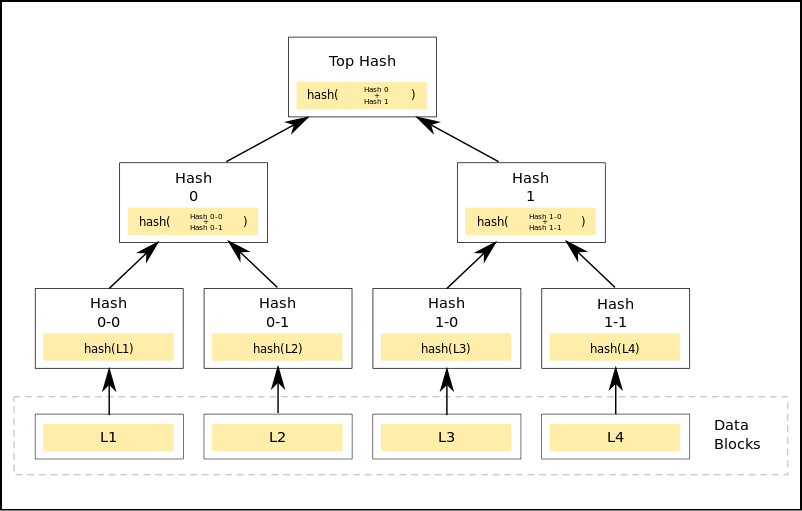
\includegraphics[width=0.9\textwidth]{merkleTree}
	\caption{Một ví dụ của cây hash nhị phân. Nguồn: Wikipedia}
	
\end{figure}

\section{Cấu trúc dữ liệu Blockchain}
Blockchain là một danh sách liên kết chứa dữ liệu và một con trỏ hash chỉ đến block trước nó, tạo thành một chuỗi (chain).

\begin{figure}[h]
	\centering
	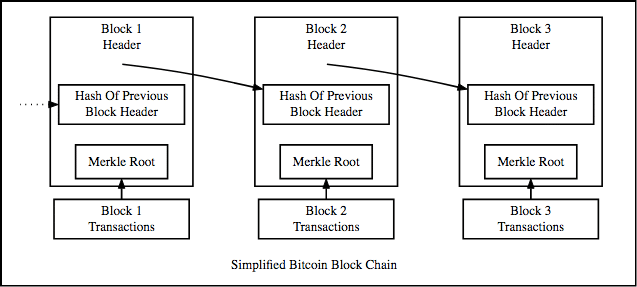
\includegraphics[width=0.9\textwidth]{blockchainStruct}
	\caption{Minh họa cấu trúc dữ liệu blockchain}
	
\end{figure}

Con trỏ hash giống như một con trỏ thường, nhưng chỉ chứa điạ chỉ của block trước nó, cũng như mã băm của dữ liệu bên trong block đó (block trước nó).

\begin{figure}[h]
	\centering
	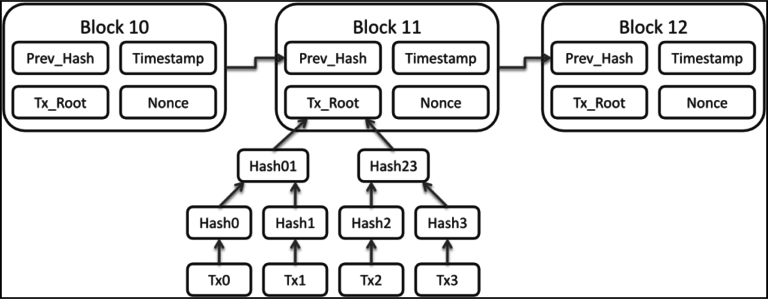
\includegraphics[width=0.9\textwidth]{blockHeader}
	\caption{Minh họa một blockheader}

\end{figure}

Một block header bao gồm:
\begin{itemize}
	\item Thời gian: timestamp hiện tại.
\item Độ khó bài toán.
\item Mã băm của block trước nó.
\item Nounce.
\item Mã băm của Merkle Root.
\end{itemize}

\chapter{Đồng thuận }

Blockchain là những hệ thống phân tán bao gồm những cá thể khác nhau hành động phụ thuộc vào động cơ 

Bất kể khi nào một giao dịch mới được đưa lện hệ thống mạng, các nút có thể lựa chọn hoặc thêm sao chép đó vào sổ cái của họ hoặc bỏ qua nó. Khi phần lớn các cá thể trong mạng đồng ý với một trạng thái (trong hai trạng thái trên),  sự đồng thuận đạt được.

Một vấn đề nền tảng trong các hệ thống điện toán phân toán và đa tác nhân là đạt được sự tin cậy tổng quát trong sự hiện diện của một số tiến trình bị lỗi. Điều này thường yêu cầu quy trình nhằm đồng thuận về một số giá trị dữ liệu cần trong quá trình tính toán.

Các quy trình này được được gọi là sự đồng thuận.

Để tạo ra một giao thức đồng thuận bảo mật,  nó phải chịu được lỗi (fault tolerant).

Để hiểu được giao thức đồng thuận trong blockchain, trước hết cần phải nói đến \textit{Bài Toán Hai Vị Tướng} (Two Generals Problem) và phiên bản mở rộng \textit{Byzantine Generals’ Problem} và thảo luận về \textit{Byzantine Fault Tolerance} trong hệ thống phân tán và phi tập trung để cuối cùng thảo luận mối liên quan của các vấn đề trên với blockchan.

\section{Bài Toán Hai Vị Tướng}

Bài toán này (lần đầu được đăng vào năm 1975 và có tên gọi trên vào năm 1978) mô tả một trường hợp khi hai vị tướng cùng tấn công một kẻ thù chung. Tướng 1 được xem như chỉ huy và tướng kia là người đi theo. Đội quân của mỗi vị tướng tự bản thân không thể đánh bại được quân đội kẻ thù, vì vậy họ cần phải phối hợp và tấn công cùng lúc. 

Để họ có thể liên lạc và quyết định thời điểm, Tướng 1 phải gửi một tin nhắn đi qua trại địch, trong đó cung cấp thời gian đợt tấn công cho Tướng 2. Vì vậy, có khả năng tin nhắn sẽ bị bắt được bởi kẻ địch và vì vậy tin nhắn sẽ không tới nơi. Điều đó sẽ dẫn đến việc Tướng 1 tấn công trong khi Tướng 2 và quân đội của ông ta đứng yên.

Ngay cả khi tin nhắn thứ nhất vượt qua được, Tướng 2 phải báo (acknowledge, ACK, tương tự như 3-way handshake của TCP) rằng ông ta đã nhận được tin nhắn, nên ông ta phả gửi một tin nhắn về, vì vậy lập lại trường hợp cũ khi tin nhắn có thể bị bắt. Điều này dẫn đến vô hạn số lần ACK và vì vậy các vị tướng không thể đạt được một sự đồng thuận.

Không có cách nào đảm bảo rằng yêu cầu thứ hai - mỗi vị tướng chắc chắn rằng bên kia đã đồng ý với kế hoạch tấn công. Cả hai vị tướng sẽ đều lo lắng rằng tin nhắn cuối cùng của họ có tới nơi hay không.

\begin{figure}[h]
	\centering
	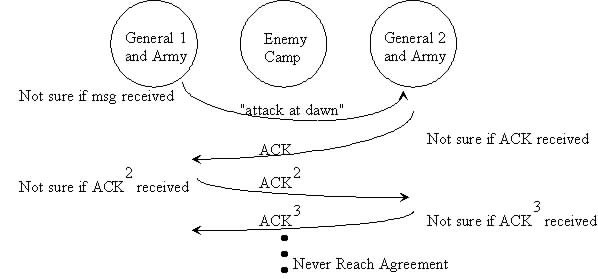
\includegraphics[width=0.9\textwidth]{twogeneral}
	\caption{Do xác suất tin nhắn không đi qua được luôn > 0, các tướng khong thể đạt được một sự đồng thuận với 100\% tin tưởng}
	
\end{figure}


Bài Toán Hai Vị Tướng đã được chứng minh là không thể giải.




%\chapter{Lịch sử blockchain}
%
%Blockchain được công chúng biết tới lần đầu tiên khi Satoshi Nakamoto, người mà danh tính thật sự  vẫn chưa ai biết, đăng bài báo cáo Bitcoin: A Peer to Peer Electronic Cash System vào năm 2008, trong đó mô tả một 'phiên bản mạng ngang hàng của tiền ảo' được gọi là Bitcoin.  Blockchain, công nghệ mà Bitcoin chạy trên  , đã phát triển trong suốt thập niên qua, thành một trong những công nghệ đột phá lớn nhất với tiềm năng tác động đến mọi ngành từ tài chính đến sản xuất. Dưới đây là một lịch sử ngắn gọn về công nghệ blockchain:
%
%\section{Khởi đầu với Bitcoin}
%Ta không thể  nói về lịch sử của blockchain mà không bắt đầu bằng việc nói về Bitcoin. Sau khi báo cáo của Nakamoto được đăng, Bitcoin được cung cấp cho cộng đồng mã nguồn mở trong năm 2009. Blockchain cung cấp giải pháp cho vấn đề sự tin tưởng trong thế giới số bởi vì bất kỳ ai cũng có thể xem thông tin mà nó ghi lại và không cho phép bất kỳ ai xóa chúng. Nó có tinh minh bạch, có ghi lại thời gian và có tính phi tập trung.
%
%%“Blockchain dùng cho Bitcoin, như internet dùng cho email. Một hệ thống điện tử lớn, mà bạn có thể xây ứng dụng trên đó. Tiền tệ chỉ là một trong số chúng” Sally Davies, FT Technology reporter.
%
%\section{Blockchain tách ra từ Bitcoin}
%
%Ngay cả ngày hôm nay, có rất nhiều người tin rằng Bitcoin và blockchain là một và như nhau, mặc dù không phải thế. Trong năm 2014, nhiều người bắt đầu nhận ra  rằng blockchain có thể được sử dụng không chỉ cho tiền mã hóa mà còn cho nhiều thứ khác nên họ bắt đầu đầu tư và nghiên cứu làm thế nào để sử dụng blockchain để thay đổi  quy trình hoạt động trong các lĩnh vực khác nhau. Cốt lõi của blockchain là một sổ cái mở, phi tập trung, ghi lại các giao dịch giữa hai bên một cách liên tục mà không cần xác thực của bên thứ ba. Điều này giúp tăng tính hiệu quả và làm giảm đáng kể chi phí giao dịch.
%
%Khi các doanh nhân hiểu được sức mạnh của blockchain, đã có một sự gia tăng đầu tư và nghiên cứu để xem làm thế nào để ứng dụng blockchain vào chuỗi cung ứng, y tế, bảo hiểm, vận chuyển, bầu cử, quản lý hợp đồng và nhiều hơn nữa. Gần 15\% các tổ chức tài chính hiện tại đang sử dụng công nghệ blockchain. 
%
%\section{Sự nổi lên của Ethereum: Hợp đồng thông minh}
%
%Vitalik Buterin, đồng sáng lập  Ethereum và tạp chí Bitocoin, cũng là một trong những người đóng góp cho hệ thống codebase Bitcoin những ngày đầu tiên, nhưng bắt đầu nản lòng trong  2013 bởi sự hạn chế về lập trình của nó và thúc đẩy cải tiến nó trở nên mềm dẻo hơn. Gặp phải sự phản đối từ cộng đồng Bitcoin, Buterin bắt đầu xây dựng một blockchain mở thứ hai gọi là Ethereum. Sự khác biệt lớn nhất giữa hai blockchain là Ethereum có thể ghi chép lại không chỉ tiền tệ mà còn các tài sản khác như là các khoản vay hoặc hợp đồng. Ethereum ra mắt vào năm 2015 và có thể được sử dụng để xây dựng “hơp đồng thông minh”—có thể tự động xử lý dựa trên một bộ quy tắc được thiết lập trong blockchain Ethereum. Công nghê này đã thu hút sự chú ý của các tập đoàn như Microsoft, BBVA và UBS, bị lôi cuốn bởi tiềm năng giúp tiết kiệm thời gian và tiền bạc của hợp đồng thông minh.
%
%\section{Sự chuyển dịch sang Proof of Stake}
%
%Hiện tại, công nghệ blockchain hoạt động dựa trên cơ chế ''chứng minh theo công sức'' (proof of work, POW): để tạo một block cần phải dùng đến khả năng tính toán của một máy tính đắc tiền. Các giao địch sẽ được đóng gói lại thành một block. Sau đó các máy đào (miner) sẽ xác nhận các giao dịch trong block có đúng với các quy tắc đề ra hay không bằng cách giải một bài toán POW, một bài toán rất khó đòi hỏi một khối lượng sức mạnh tính toán đặc biệt để giải. Máy đào đầu tiên giải được bài toán đó sẽ nhận được phần thưởng và sau đó các giao dịch được chứng thực sẽ được lưu trữ trong blockchain. Các nhà phát triển Ethereum quan tâm đến việc chuyển sang một cơ chế đồng thuận mới gọi là ''chứng minh theo cổ phần'' (proof of stake, POS).
%
%POS có  cùng mục tiêu với POW: xác nhận các giao dịch và đạt được sự đồng thuận trong chuỗi thông quan việc sử dụng một thuận toán khác.  Với POS, người tạo ra block mới ''được chọn theo một cách xác định, tùy thuộc vào lượng tài sản (trong blockchain) mà người nó nắm giữ, hay trong POS được gọi là cổ phần (stake).''  Những người ủng hộ sự thay đổi này, bao gồm đồng sáng lập Ethereum, Buterin, thích cơ chế POS do cơ chế này giúp tiết kiệm năng lượng và chi phí hơn so với POW.
%
%\section{Nhân rộng Blockchain}
%Do hiện tại, mọi máy tính trong một blockchain đều phải xử lý mọi giao dịch, nên quá trình này có thể diễn ra rất chậm. Một giải pháp nhân rộng Blockchain sẽ xác định xem cần bao nhiêu máy tính để xác thực một giao dịch mà không ảnh hưởng đến vấn đề bảo mật.
%
%Ngày nay, Bitcoin chỉ là một trong hàng trăm ứng dụng sử dụng công nghệ blockchan. Sự thay đổi của công nghệ blockchain đã trải qua một thập kỷ và ta không thể nào tiên đoán được thập kỷ kế tiếp blockchain sẽ thay đổi đến mức nào.
%\chapter{Khái niệm về blockchain}
%\section{Công nghệ sổ cái phân tán và Blockchain}
%
%\subsection{Công nghệ Sổ cái phân tán}
%Công nghệ Sổ cái phân tán (Distrubed Ledger Technology) (DLT) nhận được ngày càng nhiều sự chú ý trong những năm gần đây như một phương pháp mới giúp lưu trữ và cập nhật dữ lữu trong và giữa các tổ chức. Một sổ cái phân tán là một sổ cái số, khác biệt so với hệ thống sổ tập trung truyền thống ở hai điểm: Đầu tiên, thông tin được lưu trữ trong một mạng lưới các máy tính mà ở đó các thay đổi xảy ra với một sổ cái trong mạng sẽ được phản ánh đồng thời đến tất cả chủ sỡ hữu các sổ cái khác. Thứ hai, thông tin được xác nhận bởi một chữ ký điện tử. Những hệ thống này cùng nhau cung cấp một bản ghi giao dịch minh bạch và có thể kiểm tra lại. 
%
%\subsection{Công nghệ Blockchain}
%Công nghệ blockchain là một trong những ứng dụng được biết đến nhiều nhất của DLT, trong đó sổ cái bao gồm các khối (block) chứa các giao dịch, nó là công nghệ nền tảng của Bitcoin. Tuy nhiên, các ứng dụng khả dĩ của DLT đã lan tới lĩnh vưc giáo dục, các ngàng công nghệ sáng tạo, và các ngành nông nghiệp và thực phẩm.
%
%Những tính năng chính của Blockchain,  thứ làm nó khác biệt so với các loại cơ sở dữ liệu khác, xuất phát từ bản chất ''phân tán'' của nó. Trong blockchain, mỗi nút trong blockchan đều giữ một phiên bản sổ của riêng họ, dữ liệu được thêm vào nhờ thuật toán đồng thuận và không cần bên thứ ba. Kết quả là, Blockchain có thể cung cấp nhiều lợi ích trong các vấn đề về tính hiệu quả, niềm tin và đối chiếu dữ liệu giữa tất cả sổ cái trong blockchain. Điều này có nghĩa là Blockchin có thể cung cấp:
%\begin{itemize}
%	\item \textit{Một bản ghi không thể thay đổi được:} Dữ liệu được thêm vào sổ cái không thể thay đổi, được bảo vệ và hiện diện trong suốt vòng đời của sổ cái, nếu như được đồng thuận bởi mọi thành viên
%	 \item \textit{Khả năng phi trung gian:} Các nút có khả năng tương tác trực tiếp mà không cần đến một bên trung gian. Điều này bao gồm khả năng khởi tạo các giao dịch dữ liệu hoặc tài sản đã được số hóa (có thể là một loại tiền tệ, chẳng hạn như bitcoin, hoặc một đại diện số của tài sản thực, ví dụ như quyền sở hữu đất hoặc tiền thật).
%	\item \textit{Không bị điều khiển bởi một cá thể trung tâm:} Việc thêm dữ liệu vào sổ cái hoặc thay đổi cấu trúc điều hành phải được quyết định dựa sự đồng thuận của các bên tham gia.
%	\item \textit{Cơ hội mói cho việc quản lý và chia sẽ dữ liệu.} Việc truy cập dữ liệu giữa các bên tham gia dễ dàng hơn sẽ tạo ra nhiều ứng dụng cho việc quản lý và chia sẽ dữ liệu. 
%\end{itemize}
%
%\section{Các loại Blockchain}
%%Sổ Không Cần Cho Phép (Permisionless) hay Sổ Công Cộng (Public) được xem như một torng những dạng ''nguyên thủy nhất'' của Blockchain.  Một ví dụ điển hình chính là Blockchain, công nghệ nền tảng của Bitcoin. Trong loại cấu hình này, những người tham gia ''không cần được cho phép'' và bất kỳ ai cũng có thể tham gia và thực hiện xác thực giao dịch với đầy đủ quyền. Những người tham gia được xác định thông qua tên giả hoặc được gữ kín, 
%Một blockchain có thể là permisionless (không cần cho phép) (như Bitcoin hoặc Ethereum) hoặc permissioned (cần cho phép)). Một blockchain không cần cho phép, còn được gọi là một blockchain công cộng, bởi vì bất kỳ ai đều có thể tham gia vào mạng. Một blockchain cần cho phép, hay blockchain riêng tư, yêu cầu xác minh trước của các bên tham gia trong mạng, và các bên này thường đã biết nhau.
%
%Sự lựa chọn giữa blockchain công cộng và riêng tư thường được quyết định bởi các ứng dụng cụ thể cần gải quyết. Một ví dụ mà các doanh nghiệp trao đổi thông tin với nhau là trong quản lý chuỗi cung ứng. Quản lý chuỗi cung ứng là một trường hợp lý tưởng để sử dụng blockchain riêng tư. Ta không muốn các công ty không mời tham gia vào mạng. Mỗi bên tham gia chuỗi cung ứng sẽ được yêu cầu quyền (permission) để thực hiện các giao dịch trong blockchain. Các giao dịch này sẽ cho phép các công ty khác biết một sản phẩm cụ thể đang nằm ở đâu.
%
% Ngược lại, khi một mạng có thể tạo thuận lợi cho các bên giao dịch mà không nhất thiết phải xác minh danh tính của nhau, như blockchain Bitcoin, một blockchain công cộng phù hợp hơn. Một số ví dụ như bán hoặc phân phối sản phẩm trong một cộng đồng. Các loại tiền mã hóa (vốn không được các chính phủ ủng hộ) thường sử dụng blockchain công cộng.


%\textbf{Ví dụ của hàm băm mật mã học}
%\begin{itemize}
%	\item MD 5: Nó tạo ra một mã hash 128-bit. Collision resistance gãy vỡ sau khoảng 2\^21 hashes.
%\item SHA 1: Tạo ra một 160-bit hash. Collision resistance gãy vỡ sau khoảng 2\^{61} hashes.
%\item SHA 256: Tạo ra một 256-bit hash. Nó đang được sử dụng bởi Bitcoin.
%\item Keccak-256: Tạo ra một 256-bit hash và đang được sữ dụng bởi Ethereum.
%\end{itemize}

% \chapter{Cấu trúc của blockchain}
%\section{Cây Merkle}
%
%Cây Merkle, cũng được gọi là cây hash nhị phân, là một cấu trúc dữ liệu được dùng để lưu mã hash của từng cá thể dữ liễu  trong một tập dữ liệu (dataset) lớn nhằm giúp việc xác minh dữ liệu trở nên hiệu quả. Đây là một cơ chế chống giả mão để đảm bảo rằng tập dữ liệu lớn không bị thay đổi. Từ ''cây'' được dùng để chỉ một dạng cấu trúc dữ liệu phân nhánh, như thể hiện trong hình bên dưới. Theo Andreas M. Antonopoulos, tác giả cuốn Mastering Bitcoin, thì ''Cây Merkle được dùng để tóm tắt tất cả giao dịch trong một block, tạo ra một dấu vân tay kỹ thuật số của toàn bộ tập giao dịch, cung cấp một quy trình hiệu quả để chứng thực liệu một giao dịch nào đó có nằm trong khối hay không''
%\begin{figure}[h]
%	\centering
%	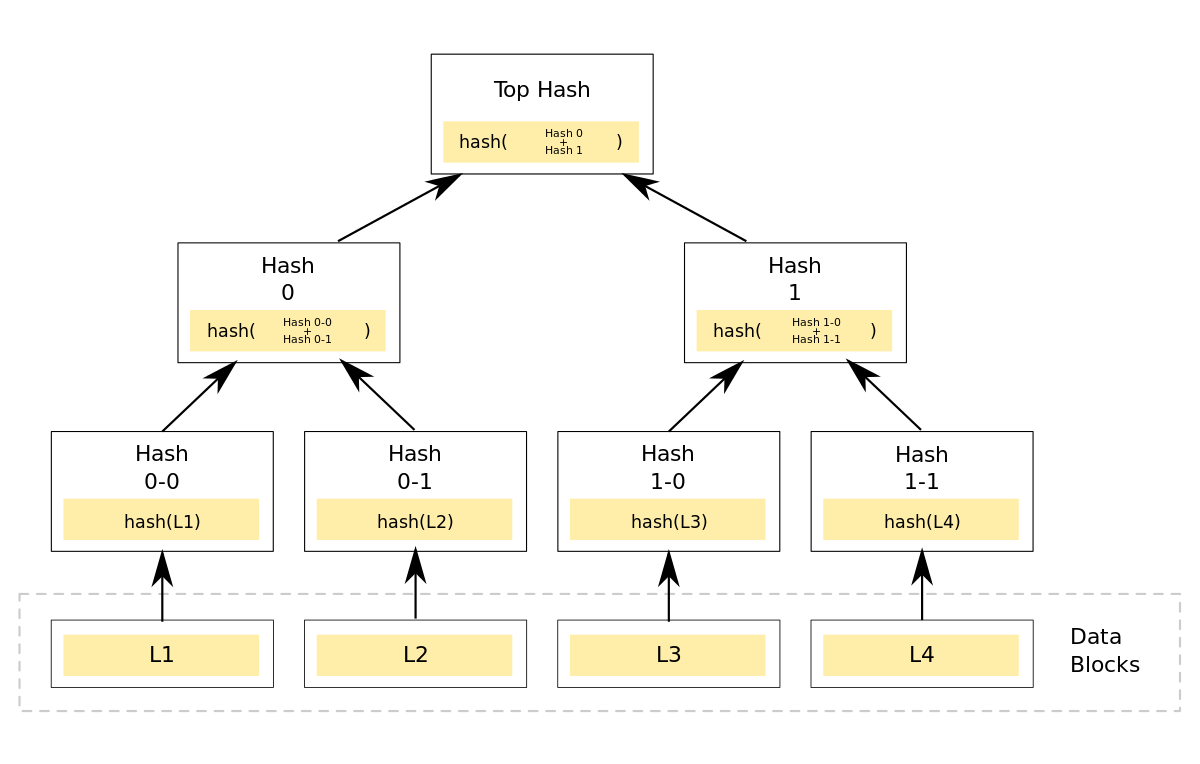
\includegraphics[width=0.9\textwidth]{Hash_Tree.png}
%	\caption{Một ví dụ của cây hash nhị phân.}
%\end{figure}
%
%\section{Block}
%
%Mỗi giao dịch trong tập giao dịch (tạo nên blockchain) được nạp vào một chương trình, tạo ra một mã được mã hóa được gọi là mã băm (hash value).\\
%Các mã băm được kết lại hợp thành một cây Merkle.\\
%Mã băm cuối cùng của tất cả quá trình băm này được đưa vào header của block, cùng với mã băm của header block trước nó và một tem thời gian.\\
%Header này sau trở thành một phần của một bài đố mật mã học có lời giải là một con số gọi là "nounce".\\
%Một khi lời giải đã được tìm ra thì block mới này sẽ được thêm vào blockchain


 






\end{document}
